%------------------------------------------------
% Quick reference. 
%------------------------------------------------
%
% Для вставки картинок:
%
%--------         Комманда
%
%\begin{figure}[H]
%	\includegraphics{img_name}
%	\caption{some caption}
%	\label{some_pic}
%\end{figure}
%
%--------        Переменные
%
% img_name     <- Название картинки в папке img.
% some_caption <- подпись картинки.
% label        <- лейбл нужен для ссылок на картинку.
% H            <- расположение картинки на странице.
%
%--------         Пример
%
%\begin{figure}[H]
%	\includegraphics{pic1.jpg}
%	\caption{График зависимости чего-то там}
%	\label{grapics1}
%\end{figure}
%
%------------------------------------------------
%
% Для референса по лейблу:
%
%--------         Комманда
%
% Для ссылки используется \eqref{ref}.
%
%--------        Переменные
%
% ref          <- указанный лейбл в директиве \label{ref}
%                 Ссылку можно сделать на любой объект имеющий \label{•}
%
%--------         Пример
%
% \eqref{graphics1}
%
% Ссылка на источники [\ref{src_spectral_wiki}]
%
%------------------------------------------------
%
% Для листинга кода:
%
%--------         Комманда
%
% \lstinputlisting[language=lang,mathescape=true]{src}
%--------        Переменные
%
% lang         <- язык на котором написан исходный код, например "python" или "C++".
% mathescape   <- если в исходниках есть формулы LaTeX, то они будут представлены как формулы.
% src          <- путь до файла исходников.
%
%--------         Пример
%
% \lstinputlisting[language=C++,mathescape=false]{./src/bullshit.cpp}
%
%------------------------------------------------
%
% Для вставки таблиц:
%
%--------
%\begin{table}[H]
%	\centering
%	\caption{ capt }
%	\begin{tabularx}{0.9\textwidth}{ | Y | Y | }
%		\hline
%		lines
%	\end{tabularx}
%	\label{tab1}
%\end{table}
%--------
% caption      <- Подпись таблицы.
% tab1         <- лейбл нужный для ссылки на таблицу.
% | Y | Y |    <- количество и формат столбцов.
% Y            <- Тип столбца.
%                 В данном случае определены кастомные столбцы Y (Спасибо Максиму Наумову)
% |            <- обозначает границы столбца.
%                 То есть, если будет указано |Y Y|, то столбцы внутри строк разделены не будут.
% H            <- То же самое, что и у картинок.
% lines        <- непосредственно элементы таблицы.
%                 Разделяются знаком "&", оканчивать каждую строку лучше \\ \hline
%
%--------         Пример
%\begin{table}[H]
%	\centering
%	\caption{ capt }
%	\begin{tabularx}{0.9\textwidth}{ | Y | Y | }
%		\hline
%		str1 & str2 \\ \hline
%		str1 & str2 \\ \hline
%		str1 & str2 \\ \hline
%		str1 & str2 \\ \hline
%		str1 & str2 \\ \hline
%	\end{tabularx}
%	\label{tab1}
%\end{table}
%------------------------------------------------

\documentclass[14pt, a4paper, fleqn]{extarticle}

\makeatletter
\renewcommand*\l@section{\@dottedtocline{1}{1.5em}{2.3em}}



%\includegraphics{universe}

\usepackage[utf8]{inputenc}
\usepackage[T2A]{fontenc}
\usepackage[russian]{babel} % указывает язык документа
\usepackage[left=3cm,right=2cm,top=2cm,bottom=2cm,bindingoffset=0cm]{geometry}
\usepackage{lastpage}
\usepackage{fancyhdr}
\usepackage{titlesec}
\usepackage{multirow}
\usepackage{graphicx} % для вставки картинок
\usepackage[intlimits]{mathtools} % математические дополнения
\usepackage{amssymb}
\usepackage[tableposition=top]{caption}
\usepackage{subcaption}
\usepackage{indentfirst}
\usepackage{pythonhighlight}
\usepackage{listings}
\usepackage{tabularx}
\usepackage{tabulary}
\usepackage{multirow}
\usepackage{xcolor,colortbl}
\usepackage{float}
\usepackage[figure,table]{totalcount}
\usepackage{diagbox}
\usepackage[german=guillemets]{csquotes}
\usepackage{fontspec} 
\usepackage{enumitem}
%\usepackage{mathptmx}% http://ctan.org/pkg/mathptmx
%\usepackage{showframe}
\usepackage{hyperref}

\setlength{\parindent}{1.2cm}

\setlength{\mathindent}{1.2cm}

\defaultfontfeatures{Ligatures={TeX},Renderer=Basic} 
\setmainfont[Ligatures={TeX,Historic}]{Times New Roman}

%\setlist[enumerate]{itemindent=\dimexpr\labelwidth+\labelsep\relax,leftmargin=0pt}

%\setlength{\section*}{0.5cm}
%\usepackage{minted}
%\usepackage{fancyvrb}
%\usepackage{newtxtext}

%\titleformat{\section}[hang]{\bfseries\LARGE\centering}{}{1em}{}

%\setlist[enumerate]{itemindent=\dimexpr\labelwidth+\labelsep\relax,leftmargin=0pt}
\setlist[enumerate,itemize]{leftmargin=0pt,itemindent=1.7cm}
\titlespacing*{\section}{0.6cm}{1ex}{1em}
\titleformat{\section}{\bfseries\centering}{\thesection}{0.5em}{\MakeUppercase}
\titleformat{\subsection}[block]{\bfseries\hspace{1em}}{\thesubsection}{0.5em}{}
%\setlength{\subsection*}{1.5cm}
%\setlength{\parindent}{4em}

%\setlength{\parindent}{1.5cm}

\captionsetup[figure]{name={Рисунок},labelsep=endash, skip=5pt}
\captionsetup[table]{name={Таблица},labelsep=endash,singlelinecheck=false, skip=5pt}


%\renewcommand{\baselinestretch}{1.5}
\linespread{1.5} % полуторный интервал
\frenchspacing
\graphicspath{ {images/} }

%-------------------------------------------
% Ссылки в оглавлении
%-------------------------------------------

\hypersetup{
    colorlinks,
    citecolor=black,
    filecolor=black,
    linkcolor=black,
    urlcolor=black
}

%-------------------------------------------
% Стиль футеров и хедеров
%-------------------------------------------

\pagestyle{fancy}
\fancyhead[L, R]{}
\fancyfoot[L]{}
\fancyfoot[R]{}
\renewcommand{\footrulewidth}{0pt}
\renewcommand{\headrulewidth}{0pt}

%\renewcommand\subsectionfont{\normalfont\normalsize\bfseries}

\def\l@subsection{\@dottedtocline{2}{3.8em}{3.2em}}
\setcounter{tocdepth}{2}
% Для листинга

\lstset{
basicstyle=\footnotesize\ttfamily,
columns=fullflexible,
keywordstyle=\color{blue},
%frame=single,
breaklines=true,
numberstyle=\tiny\color{mygray},
postbreak=\mbox{\textcolor{red}{$\hookrightarrow$}\space},
showstringspaces=false,
}

\newcolumntype{Y}{>{\centering\arraybackslash}X}

%\renewcommand{\theenumi}{\the}
\newcommand{\incpic}[3]{
	\begin{figure}[H] 
		\begin{center} 
			\includegraphics[height=0.6\textwidth]{#1} 
			\caption{#2}
			\label{#3} 
		\end{center}
	\end{figure} 
}

\begin{document}

\pagenumbering{arabic}

\setcounter{page}{3}
%\setcounter{tocdepth}{3}
\setcounter{secnumdepth}{3}

%------------------------------------------------
% Реферат
%------------------------------------------------
\phantomsection
\section*{РЕФЕРАТ}
{
	{\bf Отчет:}
	\pageref{LastPage} страницы,
	%42 страницы,
	\totalfigures\ рисунка,
	\totaltables\ таблицы,
	10 источников,
	1 приложение.
	
	%{\bf Презентация:} 19 страниц PDF.\\
	
	\textit{ОБРАБОТКА ИЗОБРАЖЕНИЙ, ДЕСКРИПТОРЫ ТОЧЕК, DAISY, PYTHON.}\\
	
	В данной работе рассмотрены алгоритмы построения дескрипторов в задачах обработки изображений.
	
	Цель работы -- разработка устойчивого к пространственным преобразованиям алгоритма построения дескрипторов.
	
	Рассмотрены принципы построения дескрипторов изображений, создана программная реализация с применением алгоритма DAISY, проведено экспериментальное исследование работы алгоритма.
}
\newpage

\newpage
\tableofcontents


%------------------------------------------------
% Введение
%------------------------------------------------
\newpage
\phantomsection
\addcontentsline{toc}{section}{Введение}
\section*{Введение}
{	
	В ряде задач цифровой обработки изображений возникает необходимость однозначного численного описания представленных на изображении точек. В частности, на численном описании отдельных точек и областей изображения основаны решения задач идентификации объектов, совмещения изображений, построения карт глубины и восстановления трехмерной сцены методами фотограмметрии, и многих других.
	
	Математические объекты, описывающие точку изображения, называют дескрипторами. Существует значительное число алгоритмов построения дескрипторов, отличающихся деталями своей реализации, скоростью и точностью работы, а также корректностю результатов для различных исходных данных. 
	
	Основными требованиями к дескриптору являются однозначность результата для одинаковых точек изображений, устойчивость к пространственным и яркостным преобразованиям исходных данных, а также вычислительная сложность алгоритмов построения. 
	
	Целью работы является разработка дескриптора изображений, устойчивого к пространственным преобразованиям.
	
	В данной работе были рассмотрены некоторые дескрипторы и алгоритмы их построения, методы программной реализации. Разработана реализация построения дескрипторов на основе алгоритма0 DAISY.  
	
	Используемые алгоритмы реализованы на языке программирования общего назначения Python 3.7 с использованием open-source библиотек для обработки изображений OpenCV версии 3.4.2 и scikit-image версии 0.6.12. В качестве тестовых данных использовались наборы изображений из ряда открытых источников.
}

\newpage

%------------------------------------------------
% Начало основной части
%------------------------------------------------
%\titleformat{\section}[runin]{\bfseries\RaggedRight\nohyphens}{\thesection}{0.5em}{}{}
\titleformat{\section}[block]{\bfseries\hspace{0.2em}}{\thesection}{0.5em}{}{}
\titleformat{\subsection}[block]{\bfseries\hspace{1.2em}}{\thesubsection}{0.5em}{}
\titleformat{\subsubsection}[block]{\bfseries\hspace{1.2em}}{\thesubsubsection}{0.5em}{}
\titlespacing*{\section}{1.1cm}{1ex}{1em}
\titlespacing*{\subsection}{0.6cm}{1ex}{1em}
\titlespacing*{\subsubsection}{0.6cm}{1ex}{1em}
\section{Исследование алгоритмов построения дескрипторов изображений}
{
\subsection{Постановка задачи}{
	Дескриптором называют математический объект, сопоставленный с определенной точкой изображения, и представляющий достаточно однозначное ее описание, позволяющее с высокой степенью уверенности идентифицировать аналогичную точку или область на другом изображении. 
	
	Как правило, дескриптор представляет собой вектор значений, вычисляемый определенной функцией для точки изображения.
	
	Стоит заметить, что на практике для однозначного описания точки изображения недостаточно исключительно информации о яркости отдельного пикселя. В связи с этим, в качестве исходных данных для построения дескриптора используется набор из нескольких точек изображения, находящихся в окрестности заданной.  
	
	Рассмотрим следующую постановку задачи.
	Обозначим дескриптор точки $p$ как $d_p$.
	Пусть дано изображение:
	\begin{equation}\label{problem_images}
	I : S \rightarrow \mathbb{R}, \quad S \subset \mathbb{R}^k,
	\end{equation}
	   	\begin{tabular}{ rl }
	  	 \quad \quad где 
	   	& $k$ -- размерность, для плоских изображений равная 2.
	   	\end{tabular}\\
   
	Построение дескриптора будет выглядеть следующим образом:
	\begin{equation}\label{problem_transform}
	d_p = f(I(\hat{p})), \quad \hat{p} \in S.
	\end{equation} 
	   	\begin{tabular}{ rl }
	   	\quad \quad где 
	   	& $f$ -- функция построения дескриптора, \\
	   	& $\hat{p}$ -- набор точек изображения $I$.
	\end{tabular}\\

	Данная схема сохраняется независимо от конкретного алгоритма построения дескриптора. Конкретный вид и свойства полученного результата будут зависеть как от вида функции $f$, так и от конфигурации набора исходных точек $\hat{p}$.
 
	Основным требованием к дескриптору является однозначность результата, т.е. удовлетворение значения \eqref{problem_transform}  следующему выражению для произвольного числа изображений $N$:
	\begin{equation}\label{problem_constraints}
	f(I_i(\hat{p_i})) = f(I_j(\hat{p_j})), \quad i=1 \hdots N, \quad j=1 \hdots N,
	\end{equation} 
	\begin{tabular}{ rl }
	\quad \quad где 
	& $p_i, p_j$ -- пара соответствующих точек изображений $I_i$, $I_j$.
	\end{tabular}\\

	Следует заметить, что построенные дескрипторы, как правило, подвергаются нормализации для уменьшения влияния на точность идентификации точек яркостных характеристик изображения и пространственных преобразований. Конкретные методы нормализации будут рассмотрены в следующих разделах. 
	
	Таким образом, используя различные функции построения и варьируя набор исходных точек, можно получать дескрипторы, обладающие различными свойствами, достоинствами и недостатками для конкретных задач. 
	
	Основными факторами, принимаемыми в расчет при разработке алгоритма построения дескрипторов, являются:
	\begin{enumerate}
	   	\item Устойчивость к пространственным преобразованиям - сохранение значения дескриптора при повороте, сдвиге, масштабировании изображения;
	   	\item Устойчивость к яркостным преобразованиями - сохранение значения дескриптора при изменении яркости и контрастности;
	   	\item Вычислительная сложность построения;
	   	\item Информативность - достаточность данных дескриптора для дальнейшей идентификации и сравнения точек.
	\end{enumerate} 

	Существует значительное число реализаций алгоритмов построения дескрипторов. Рассмотрим наиболее популярные подходы.

\subsection{Существующие алгоритмы построения дескрипторов}{
	
	Следует отметить разницу в требованиях к алгоритму построения дескрипторов в зависимости от предметной области применения. В случае использования дескрипторов для описания особых точек (features) необходима повышенная точность идентификации и инвариантность к преобразованиям, вычислительная сложность же не является самым важным критерием, т.к. число особых точек на изображении, как правило, на порядки меньше его размерности. 
	
	Напротив, в задачах плотного сопоставления изображений, возникающих в фотограмметрии и построении карт глубины, требуется вычисление дескриптора для каждого пикселя, что накладывает дополнительные ограничения на вычислительную сложность. При этом точностью построения и идентификации возможно в некоторой степени пренебречь, т.к. в данных задачах дескрипторы применяются для оценки общих тенденций преобразований между изображениями, что позволяет за счет их большого количества добиться хороших результатов усреднением и дополнительной валидацией.
	
	SIFT, SURF, ORB. Все сосут, ибо тяжелые, хороши для фичей, плохи для dense. Отъебитесь от меня пожалуйста, спасибо.
}

\newpage

\section{Разработка алгоритма построения дескрипторов изображений}
{
	\subsection{Алгоритм построения дескрипторов}
	{
		В качестве основы для разрабатываемого метода используется алгоритм DAISY.
		В основе алгоритма лежит метод построения карт ориентации градиентов. 
		
		Картой ориентации градиента (Gradient Orientation Map) называют градиент изображения, построенный в определенном направлении. Результатом построения градиента является изображение с выделенными краями объектов, и в целом выраженными областями перепадов яркости. 
		
		Ориентация градиента в определенном направлении делает более выраженными перепады яркости изображения в этом направлении. Сказал как боженька. 
		
		Построенные карты градиентов подвергаются последовательному размытию с постепенным увеличением ядра гауссовского фильтра. Полученные карты называются свернутыми картами ориентации (Convolved Orientation Maps).
		
		Таким образом, получается набор изображений, каждое из которых с увеличением уровня размытия представляет собой все более обобщенную информацию о градиенте яркости исходного изображения. 
		
		Описанные операции выполняются один раз при начале работы алгоритма, полученные COM далее используются для семплирования результатов. 
		
		Сэмплирование результатов для каждой точки производится по следующему принципу:
		
		КАРТИНКА ТУТА
		
		Для каждой указанной на схеме точки сэмплируются значения COM, начиная с наименьшей степени размытия и заканчивая максимальной. 
		
		Полученный вектор значений нормализуется. 
		
		Полный дескриптор получается путем конкатенации всех нормализованных векторов значений COM, начиная с центральной точки. 
		
		При необходимости может производиться нормализация полного дескриптора одним из описанных способов. 
		
		Each circle represents one histogram region, which is part of the descriptor vector. Each histogram represents the Gradient Orientations (GOs) within this region. The gradient is split into $H$ discrete orientations, so each single histogram has $H$ entries.
		
		Algortihm uses $Q$ rings around the central point, on which the COMs are sampled, each ring has $T$ histograms.
		
		Therefore, each descriptor has $D_s=(Q \centerdot T+1)\centerdot H$ entries.
		
		To compute GOs at a specified point $(u,v)$, several oriented derivatives of image $I$ are computed as following:
		
		$$G_o^\sigma = G^\sigma * \left(\dfrac{dI}{do}\right)^+ , \left(\dfrac{dI}{do}\right)^+ = max\left(\dfrac{dI}{do}, 0\right),$$
		where $ G^\sigma $ is a Gaussian kernel with standard deviation $ \sigma $ and $o$ is a derivative orientation.
		
		The results $G_o^{\sigma}$ are referred as Convolved Orientation Maps (COMs).
		
		In the next step the vector $h_\sigma(u,v)$ is being built as following:
		
		$$h_\sigma(u,v) = \left[G_1^\sigma(u,v), \dots, G_H^\sigma(u,v)\right]^T$$
		
		Vector $h(u,v)$ is then normalized to unit norm. It represents the values of all the GOs at a point $(u,v)$ after convolution with a Gaussian kernel with a standard deviation $\sigma$.
		
		The full DAISY descriptor for location $(u_0,v_0)$ is defined as a simple concatenation of all the vectors $h_{\sigma i}(u,v)$ for all points beginning with the center:
		
		$$D(u_0,v_0) = [h_{\sigma 1}(u_0, v_0), h_{\sigma 1}(I_1(u_0, v_0, R_1)), \dots, h_{\sigma 1}(I_T(u_0, v_0, R_1),$$ 
		$$h_{\sigma 2}(I_1(u_0, v_0, R_2)), \dots, h_{\sigma 2}(I_T(u_0, v_0, R_2),$$
		$$\dots \dots$$
		$$h_{\sigma Q}(I_1(u_0, v_0, R_Q)), \dots, h_{\sigma Q}(I_T(u_0, v_0, R_Q)],$$
		
		where $I_j(u, v, R)$ is the location with distance $R$ from $(u, v)$ in the direction given by $j$
		when the directions are quantized into the $T$ values.
	}
	\newpage
   	\subsection{Программная реализация}{
   		
   		Алгоритм сшивки изображений для исследования был реализован на языке Python 3.7 с использованием библиотеки OpenCV 3.4.2. 
   		
   		Функция, осуществляющая процедуру совмещения, принимает на вход два изображения и тип используемого дескриптора. 
   		Используются дескрипторы SIFT, SURF, ORB, BRIEF. Заметим, что алгоритмы SIFT и SURF являются патентованными, и не присутствуют в стандартной библиотеке OpenCV из-за лицензионных ограничений. Данные алгоритмы доступны в пакете xfeatures2d при использовании версии библиотеки, включающей неофициальные алгоритмы, opencv-contrib. Использование данных алгоритмов разрешается только в некоммерческих целях [\ref{cv docs}]. 
   		
   		Для вычисления дескрипторов производится преобразование исходных изображений в градации серого.
   		
   		\begin{lstlisting}[frame=single,language=Python,mathescape=true] 
   		# convert the image to grayscale
   		gray = cv2.cvtColor(image, cv2.COLOR_BGR2GRAY)
   		\end{lstlisting}
   		
   		Производится поиск наборов особых точек при помощи выбранного дескриптора.
   	
   		\begin{lstlisting}[frame=single,language=Python,mathescape=true] 
   		# detect keypoints in the image
   		detector = cv2.FeatureDetector_create("SIFT")
   		kps = detector.detect(gray)
   		
   		# extract features from the image
   		extractor = cv2.DescriptorExtractor_create("SIFT")
   		(kps, features) = extractor.compute(gray, kps)
   		\end{lstlisting}
   		
   		Найденные наборы проверяются на совпадение дескрипторов методом knn. Полученные совпадения дополнпительно тестируются на предмет нахождения расстояния между точками в заданных пределах. Пары, прошедшие тест, используются для вычисления преобразования.
   		
   		\begin{lstlisting}[frame=single,language=Python,mathescape=true] 
   		# compute the raw matches and initialize the list of actual
   		# matches
   		matcher = cv2.DescriptorMatcher_create("BruteForce")
   		rawMatches = matcher.knnMatch(featuresA, featuresB, 2)
   		matches = []
   		
   		# loop over the raw matches
   		for m in rawMatches:
   		# ensure the distance is within a certain ratio of each
   		# other (i.e. Lowe's ratio test)
   		if len(m) == 2 and m[0].distance < m[1].distance * ratio:
   		matches.append((m[0].trainIdx, m[0].queryIdx))
   		\end{lstlisting}
   		
   		После нахождения совпавших точек, по их наборам для каждого изображения вычисляется матрица проективного преобразования.
   		Если совпавших опорных точек найдено меньше, чем четыре, проективное преобразование не может быть вычислено, и функция возвращает статус ошибки.
   		
   		\begin{lstlisting}[frame=single,language=Python,mathescape=true]
   		 # compute the homography between the two sets of points
   		(H, status) = cv2.findHomography(ptsA, ptsB, cv2.RANSAC,
   		reprojThresh)
   		\end{lstlisting}
   		
   		Построенная матрица проективного преобразования применяется ко второму входному изображению, трансформируя его до совпадения положений опорных точек.
   		
   		Исходное первое изображение и преобразованное второе записываются в одно результирующее. В зависимости от требуемых параметров, сложение может производиться с различными значениями альфа-канала, в том числе с выделением яркостью пересекающейся области либо одного из изображений в целях повышения наглядности.
   		
   		Функция возвращает результирующее изображение и отчет о работе алгоритма, включающий время выполнения и построенную матрицу проективного преобразования.
   		
   		Полный код функции представлен в приложении А.
   	}
   
   	\newpage
   	\subsection*{3.2 \quad Экспериментальное исследование работы алгоритма}{
   		\addcontentsline{toc}{subsection}{3.2\qquad Экспериментальная оценка влияния цифровых шумов на качество работы алгоритма}
   		Выбранные для исследования цифровые шумы реализованы в виде отдельных функций, принимающих на вход изображение, подлежащее зашумлению, и параметры шума. Исходный код функций зашумления представлен в приложении А.
   		
   		В качестве оценочных параметров точности работы алгоритма были выбраны общее количество найденных особых точек, процент совпадений от общего числа и смещение преобразованного изображения относительно истинного положения в результате неточности построенной матрицы проективного преобразования.
   		Количество найденных точек возвращается функцией сшивки после успешного завершения работы. Смещение относительно истинного положения вычисляется по координатам углов исходного и преобразованного изображений, оценочными параметрами смещения выступают медиана и максимум расстояний между соответствующими углами в пикселях. 
   		
   		Результаты экспериментов сохраняются в виде текстовых отчетов и (или) изображений, доступных для дальнейшего анализа и визуализации.
   		
   		Для приведенных экспериментов вторым изображением, поступающим на вход алгоритма сшивки, выступала программно вырезанная прямоугольная часть центральной области первого изображения, равная 25 процентам его площади. Такой подход, в отличии от аналогичного практическому применению алгоритма использования частично пересекающихся фотографий, позволяет гарантировать нахождение максимального принципиально возможного количества совпадающих точек, а также упростить расчет смещения и визуализацию.
   		\newpage
%   		\begin{enumerate}[label=\arabic*)]%[label=\textbf{\arabic*}.]
   			\subsubsection{ Сравнение работы алгоритмов при применении размытия } Размытие изображения, строго говоря, не является цифровым шумом, хотя и может быть достаточно распространенным дефектом фотографии. Тем не менее, размытие хорошо подходит для общего сравнения алгоритмов, так как является стационарным и легко воспроизводимым процессом понижения качества картинки. 
   			
   			В данном эксперименте входное изображение размывалось с итеративным увеличением размера ядра гауссовского фильтра $m$. Эксперимент прекращался, когда число найденных опорных точек становилось меньше четырех. Входные изображения приводились к размеру в 512 пикселей по горизонтали. На рисунках \ref{blur_sample 1}-\ref{blur sample 2} представлены примеры результатов работы программы.
   			
   			\newpage
   			\begin{figure}[H]
   				\centering                             
   				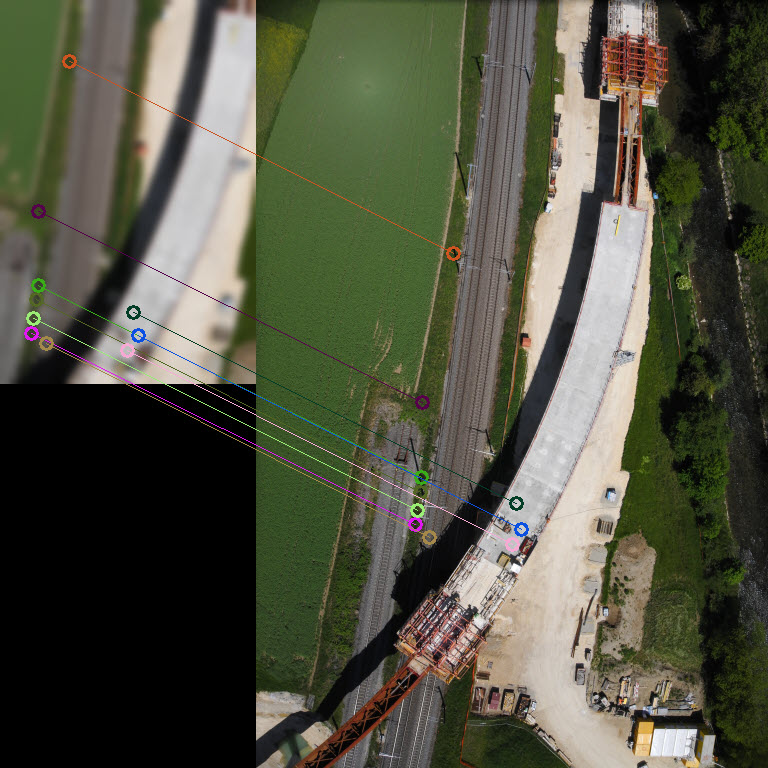
\includegraphics[width=0.65\textwidth,keepaspectratio]{samples/blur_matches.jpg}   
   				\centering\caption{ Пример отображения программой совпадений особых точек на размытом изображении }
   				\label{blur_sample 1}                           
   			\end{figure}    
   		
	   		\begin{figure}[H]
	   			\centering                                
	   			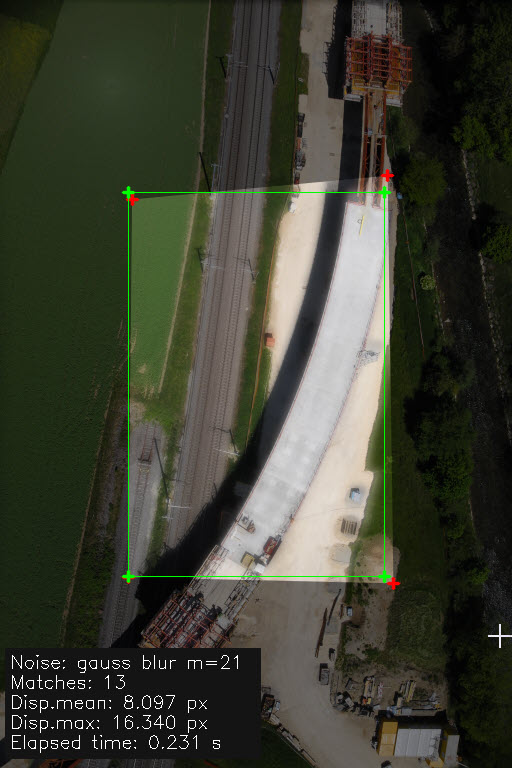
\includegraphics[width=0.45\textwidth,keepaspectratio]{samples/blur_result.jpg}       
	   			\centering\caption{ Пример отображения программой результата совмещения}
	   			\label{blur sample 2}                           
	   		\end{figure}    
   			\newpage
   			
   			\begin{table}[H]                               
   				\centering                                  
   				\caption{ Сравнение числа найденных точек при увеличении уровня размытия }                            
   				\begin{tabularx}{\textwidth}{ | c | Y | Y | Y | }
   					\hline                     
   					\multirow{2}{*}{m} & \multicolumn{3}{c}{Алгоритмы} \vline \\ \cline{2-4} 
   					&     SIFT &  SURF &  ORB  \\ \hline                           
   					- &  496  &  996 & 1286 \\ \hline
					3 &  276  &  481 & 685 \\ \hline   		
					7 &  93  &  187 & 237 \\ \hline 
					11 &  51  &  87 & 106 \\ \hline  
					17 &  25  &  48 & 23 \\ \hline 	
					19 &  21  &  42 & 17 \\ \hline 			
					21 &  16  &  30 & 9 \\ \hline 
					27 &  9  &  22 & - \\ \hline
					35 &  6  &  16 & - \\ \hline
					41 &  7  &  8 & - \\ \hline	
					49 &  5  &  6 & - \\ \hline	
					53 &  5  &  - & - \\ \hline			
   				\end{tabularx}
   				\label{ex1_count}                                
   			\end{table}           
   		
   			Прочерком обозначены значения, при которых алгоритм находит менее четырех совпадающих опорных точек.
   		
   			\begin{table}[H]                               
   				\centering                                  
   				\caption{ Сравнение медианы смещения при увеличении уровня размытия }                            
   				\begin{tabularx}{\textwidth}{ | c | Y | Y | Y | }
   					\hline                     
   					\multirow{2}{*}{m} & \multicolumn{3}{c}{Алгоритмы} \vline \\ \cline{2-4} 
   					&   SIFT &  SURF &  ORB  \\ \hline                           
   					- &  0,032  &  0,000 & 0,130 \\ \hline
   					3 &  0,082  &  0,085 & 0,163 \\ \hline
   					7 &  0,146  &  0,170 & 2,670 \\ \hline
   					11 &  0,270  &  0,303 & 1,953 \\ \hline
   					17 &  0,917  &  1,100 & 2,852 \\ \hline
   					19 &  0,405  &  1,476 & \cellcolor{blue!25} 15,543 \\ \hline
   					21 &  2,243  &  2,893 & \cellcolor{blue!25} 336,972 \\ \hline 	
   					27 &  5,564  &  1,012 & \cellcolor{blue!25} - \\ \hline		
   					35 & \cellcolor{blue!25} 13,711  &  5,951 & \cellcolor{blue!25} - \\ \hline	
   					41 & \cellcolor{blue!25} 44,210  & \cellcolor{blue!25} 10,701 & \cellcolor{blue!25} - \\ \hline
   					49 & \cellcolor{blue!25} 84,046  & \cellcolor{blue!25} 22,116 & \cellcolor{blue!25} - \\ \hline	
   					53 & \cellcolor{blue!25} 120,100  & \cellcolor{blue!25} - & \cellcolor{blue!25} - \\ \hline	
   				\end{tabularx}
   				\label{ex1 disp}                                
   			\end{table}       
   		
   			В таблице \ref{ex1 disp} цветом выделены значения медианы смещения в более чем 10 пикселей, как выбранный критерий хорошо различимого визуально показателя недостаточной точности. Прочерком обозначены значения, при которых алгоритм находит менее четырех совпадающих опорных точек.
   			
   			Результаты эксперимента отражены на рисунке \ref{blur_mch_disp}.
   			
   			\begin{figure}[H]
   				\centering                             
   				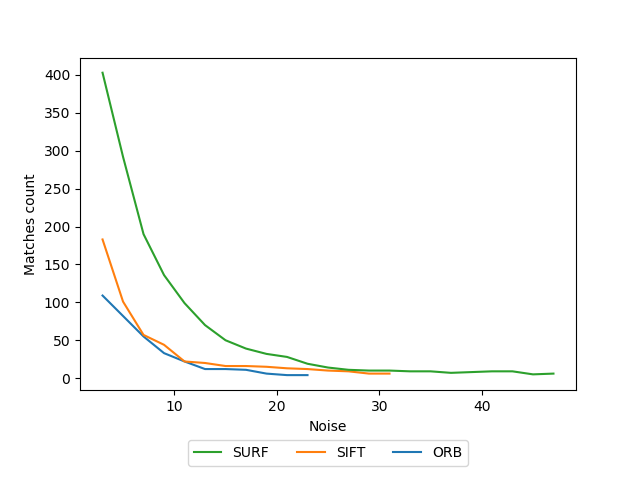
\includegraphics[width=0.75\textwidth,keepaspectratio]{ex1/Rand_noises_matches.png}   
   				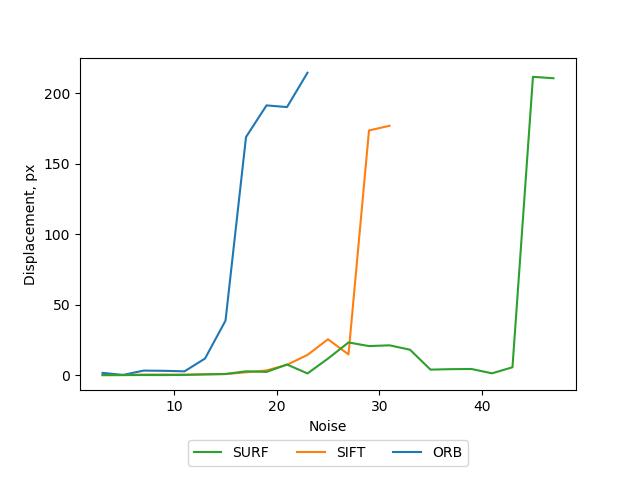
\includegraphics[width=0.75\textwidth,keepaspectratio]{ex1/Rand_noises_displacement.png}       
   				\centering\caption{ Поведение числа совпадений точек и смещения при размытии изображения }
   				\label{blur_mch_disp}                           
   			\end{figure}    
   			
   			\newpage
   			\subsubsection{ Сравнение работы алгоритмов при применении случайных шумов } При использовании случайных шумов эксперимент производился несколько раз для каждого уровня зашумленности с усреднением результатов для устранения флуктуаций и получения более общей картины. 
   			
   			Для каждого уровня зашумленности значения усреднялись по 30 экспериментам. Варьируемыми параметрами шумов выступали стандартное отклонение $\sigma$ для гауссовского шума и вероятность $p$ для шума соль-и-перец. Эксперимент прекращался, когда число найденных опорных точек становилось меньше четырех. Входные изображения приводились к размеру в 512 пикселей по горизонтали.
   			
   			Результаты экспериментов отражены на рисунках \ref{rand_noises_gauss}-\ref{rand_noises_sp}. 
   			
   			\begin{figure}[H]
   				\centering                             
   				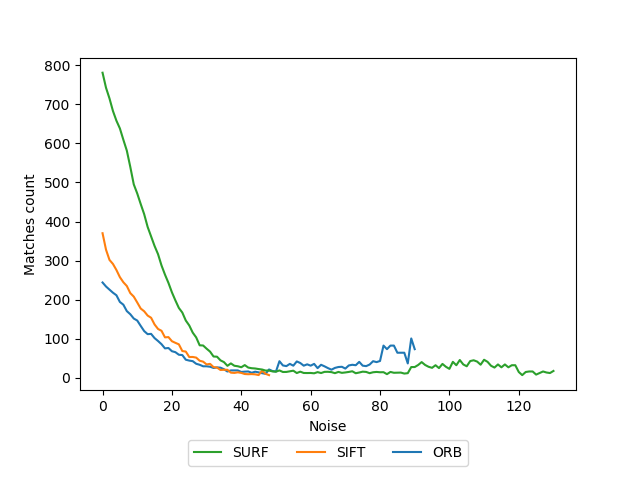
\includegraphics[width=0.75\textwidth,keepaspectratio]{ex2/gauss/Rand_noises_matches.png}   
   				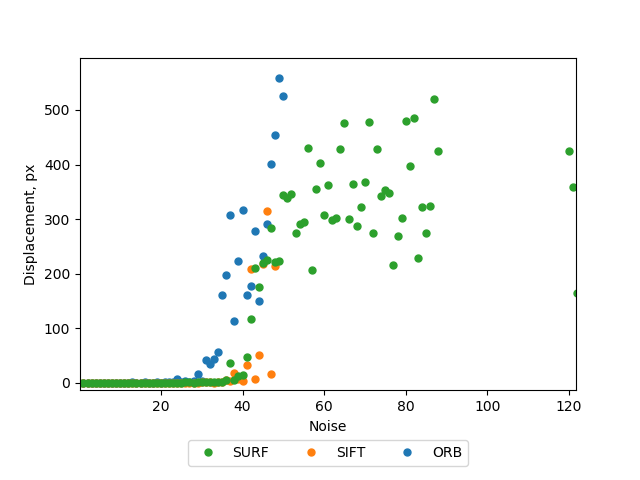
\includegraphics[width=0.75\textwidth,keepaspectratio]{ex2/gauss/Rand_noises_displacement.png}       
   				\centering\caption{ Поведение числа совпадений точек и смещения при использовании гауссовского шума }
   				\label{rand_noises_gauss}                           
   			\end{figure}    
   		
   			\begin{figure}[H]
   				\centering                             
   				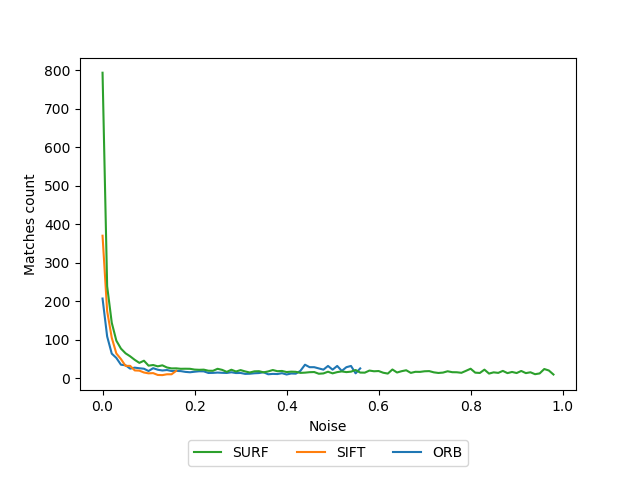
\includegraphics[width=0.75\textwidth,keepaspectratio]{ex2/sp/Rand_noises_matches.png}   
   				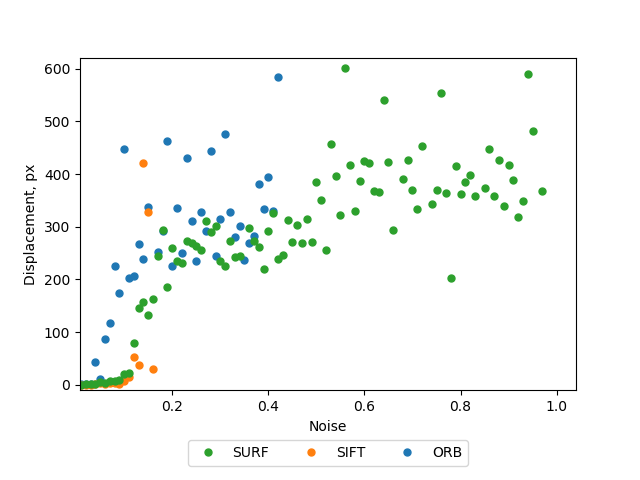
\includegraphics[width=0.75\textwidth,keepaspectratio]{ex2/sp/Rand_noises_displacement.png}       
   				\centering\caption{ Поведение числа совпадений точек и смещения при использовании шума соль-и-перец}
   				\label{rand_noises_sp}                           
   			\end{figure}   
   			
%   		\end{enumerate}	
}
}

\newpage
\section{Анализ полученных результатов}
{
    Проанализируем полученные результаты. Эксперименты показывают несколько интересных факторов в работе алгоритмов. 
    
    При размытии изображения дескриптор ORB раньше других рассмотренных начинает терять точность, несмотря на значительно большее общее количество найденных совпадений. Серьезное искажение результата достигается при размерах ядра Гауссова фильтра более 17 для тестового изображения размером 512 на 512 пикселей, с дальнейшим увеличением размера ядра ORB первым перестает находить достаточное число точек. Наилучшим образом при работе с размытым изображением показывает себя дескриптор SURF.
    
    У всех рассмотренных алгоритмов наблюдается резкое увеличение искажения результата при переходе определенного порогового значения размытия.
    
    На графике \ref{blur d by m} можно наблюдать резкое падение качества при числе точек, меньшем чем 20. Это объясняется тем, что размытие может сильно ухудшать точность определения координат особых точек, даже при сохранении общей яркостной картины достаточном для построения дескриптора. Соответственно, при малых количествах точек, ошибки в отдельных координатах сильно влияют на построенную матрицу преобразования.
    
    \begin{figure}[H]
    	\centering                             
    	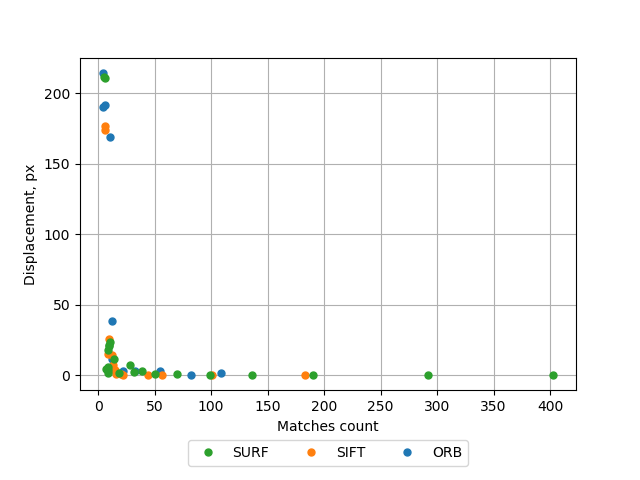
\includegraphics[width=0.75\textwidth,keepaspectratio]{ex1/Rand_noises_d_by_m.png}      
    	\centering\caption{  Изменение смещения с ростом числа точек при использовании размытия}
    	\label{blur d by m}    
	\end{figure} 
	
	При применении случайных шумов можно наблюдать более интересную картину. При использовании дескриптора SIFT точность падает равномерно, алгоритм перестает работать на тестовых изображениях при значении $\sigma$ гауссовского шума более 50 и при вероятности шума соль-перец более 0.15. При этом, остальные дескрипторы продолжают работать при значительно большем зашумлении, но стремительно теряют в точности, приводя к абсолютно непригодным для практического применения результатам. На рисунке \ref{fail surf} приведен пример результата, выданного алгоритмом SURF на значениях, при которых SIFT перестает работать. 
	
	\begin{figure}[H]
		\centering                             
		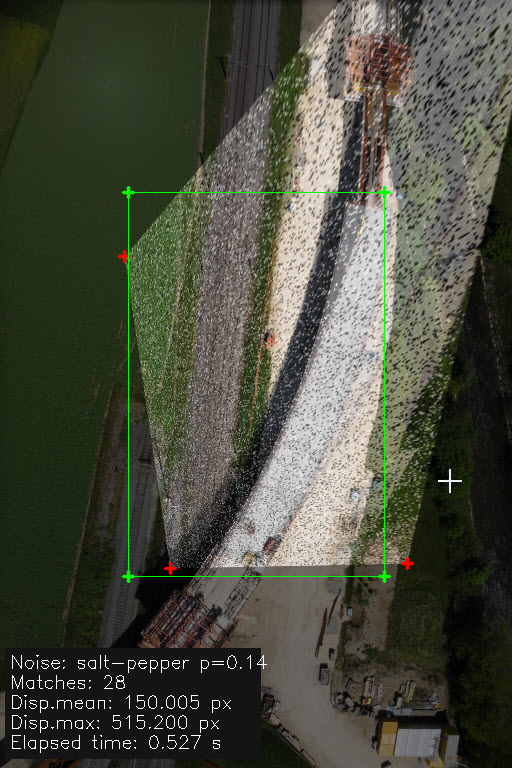
\includegraphics[width=0.45\textwidth,keepaspectratio]{fails/result.jpg}      
		\centering\caption{Пример искажения при использовании алгоритма SURF}
		\label{fail surf}    
	\end{figure} 

	Принимая во внимание практическую непригодность изображений с подобными уровнями шумов и искажений, можно отбросить диапазоны значений за пределами стабильной работы алгоритма SIFT. На графиках \ref{gauss disp big}-\ref{sp disp big} можно наблюдать этот диапазон. 
	
	\begin{figure}[H]
		\centering                             
		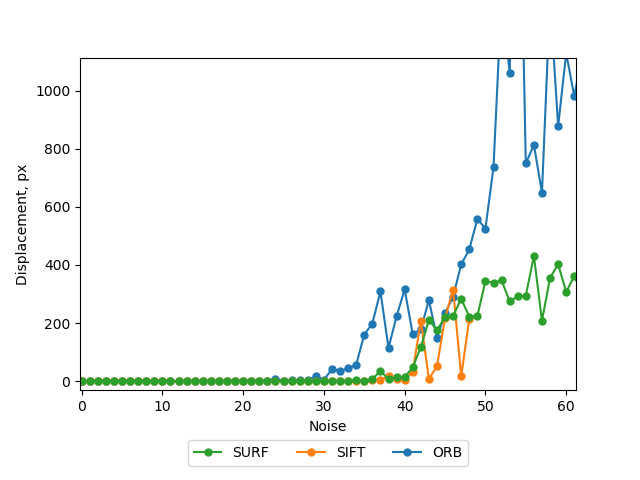
\includegraphics[width=0.60\textwidth,keepaspectratio]{ex2/gauss/Rand_noises_displacement_big.png}   
		\centering\caption{ Увеличенный фрагмент графика смещения при использовании гауссовского шума }
		\label{gauss disp big}                           
	\end{figure}    

	\begin{figure}[H]
		\centering                             
		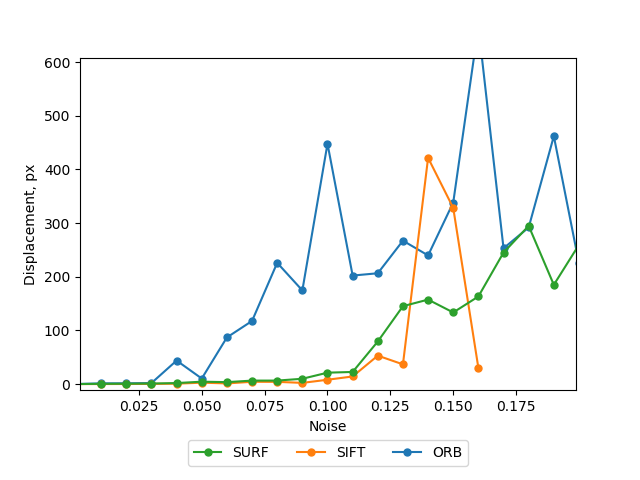
\includegraphics[width=0.60\textwidth,keepaspectratio]{ex2/sp/Rand_noises_displacement_big.png}       
		\centering\caption{ Увеличенный фрагмент графика смещения при использовании шума соль-перец }
		\label{sp disp big}                           
	\end{figure}    
	
	Как можно видеть, все три алгоритма сохраняют достаточную точность при практически достижимых уровнях гауссовского шума. Однако, ORB наименее устойчив к шуму соль-и-перец, что можно видеть по резкому пику на графике при вероятности 0.03, сохраняющемуся даже при усреднении по набору экспериментов.
	
	\begin{figure}[H]
		\centering                             
		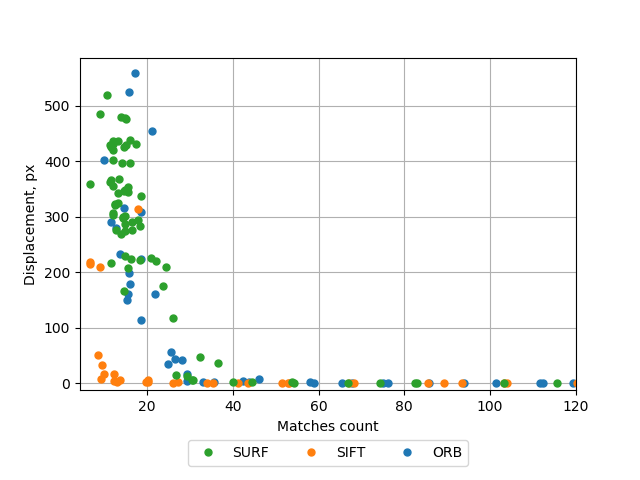
\includegraphics[width=0.6\textwidth,keepaspectratio]{ex2/gauss/Rand_noises_d_by_m.png}      
		\centering\caption{ Изменение смещения с ростом числа точек при использовании гауссовского шума}
		\label{rand_noises_gauss_b_by_m}                           
	\end{figure} 
	
	\begin{figure}[H]
		\centering                             
		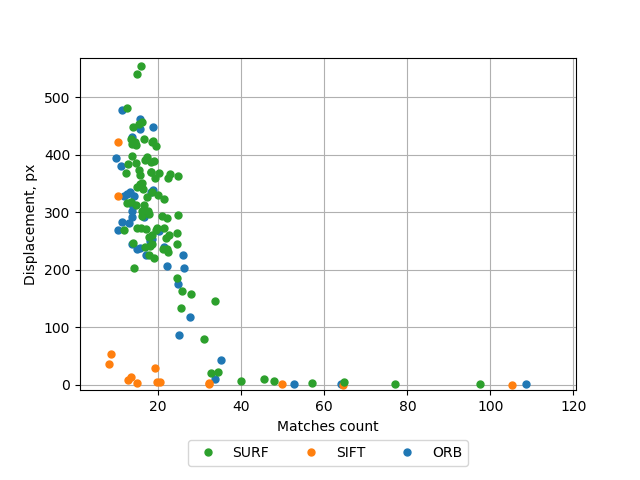
\includegraphics[width=0.6\textwidth,keepaspectratio]{ex2/sp/Rand_noises_d_by_m.png}      
		\centering\caption{  Изменение смещения с ростом числа точек при использовании шума соль-и-перец}
		\label{rand_noises_sp_b_by_m}                           
	\end{figure} 
	
	Зависимость смещения от количества найденных точек, как видно на графиках \ref{rand_noises_gauss_b_by_m}-\ref{rand_noises_sp_b_by_m}, выражена не так ярко, как при размытии, и можно наблюдать более плавный переход.
	
	Итак, наивысшая точность при применении случайных шумов достигается при использовании алгоритма SIFT. Наихудший результат показывает ORB. Стоит заметить, что и при использовании импульсного шума соль-перец, и при использовании аддитивного гауссовского шума наибольшие количества особых точек находит алгоритм SURF.
	
	Обобщая полученные результаты, можно сказать, что все рассмотренные алгоритмы проявили себя достаточно хорошо при тех уровнях зашумления, которые потенциально могут встретиться на практике. Значения, при которых наблюдается серьезное смещение относительно требуемого, в любом случае сделали бы на практике такую фотографию непригодной к использованию. 
	
	При размытии изображения наилучшим образом ведет себя алгоритм SURF, что позволяет рекомендовать его к использованию, если исходные фотографии сделаны с заметным нарушением фокусировки.
	При случайных шумах, как аддитивном, так и импульсном, наилучшим образом работает SIFT, ценой большего времени выполнения и вычислительной сложности. 
	Хуже всего в проведенных экспериментах отработал алгоритм ORB, в особенности, при использовании шума соль-перец.
}
\newpage


%------------------------------------------------
% Заключение
%------------------------------------------------

\titleformat{\section}{\large\bfseries\centering}{\thesection}{0.5em}{\MakeUppercase}
\titleformat{\subsection}[block]{\bfseries\hspace{1em}}{\thesubsection}{0.5em}{}

\newpage
\phantomsection
\addcontentsline{toc}{section}{Заключение}
\section*{Заключение}
{
    В ходе данной работы была рассмотрена задача сшивки изображения и методы ее решения. Проведен обзор математической постановки задачи. Рассмотрен алгоритм нахождения пространственного преобразования по опорным точкам. Был дан обзор нескольких методов поиска опорных точек, реализованных в открытой библиотеке OpenCV.
    
    Рассмотрены цифровые шумы в задачах обработки изображений и их особенности, разобраны популярные математические модели искусственно генерируемых шумов, используемых для тестирования алгоритмов и оборудования. 
    
    Реализована компьютерная программа, осуществляющая совмещение изображений по особым точкам с возможностью выбора типа дескриптора. Также, реализована программная среда для экспериментов, позволяющая использовать изображения с генерацией различных типов и уровней зашумления, формировать отчеты о работе алгоритмов и анализировать графическое представление результатов. 
    
    В ходе серии экспериментов было выяснено, что представленные алгоритмы являются достаточно устойчивыми к зашумлению, и работают с достаточной точностью при уровнях шума, допускающих сохранение практической ценности таких изображений. Однако, можно выделить алгоритмы, лучше или хуже ведущие себя при определенных типах шумов. Результаты экспериментов показывают, что наилучшим образом все представленные алгоритмы справились с размытием, наихудшим - с импульсным шумом. Были сделаны выводы о применимости отдельных алгоритмов при конкретных практически возможных дефектах фотографий. 
    
    Дальнейшим развитием работы видится оценка при использовании на зашумленных изображениях восстанавливающих фильтров, либо восстановления шума при помощи моделей глубокого обучения.
}

\newpage
\phantomsection
\addcontentsline{toc}{section}{Список использованных источников}
%------------------------------------------------
% Список литературы
%------------------------------------------------
\section*{Список использованных источников}
{
	\begin{enumerate}[label=\arabic*]
%	\item{Гонсалес Р., Вудс Р. Цифровая обработка изображений // М.: Техносфера. – 2005. – Т. 1072. – С. 2.}
	\item{Bres, S. Detection of interest points for image indexation [Текст] / S. Bres, J. M. Jolion // International Conference on Advances in Visual Information Systems. -- Springer, Berlin, Heidelberg, 1999. -- P. 427-435.}{\label{interest points}}	
	\item{Lowe, D. G. Distinctive image features from scale-invariant keypoints [Текст] / D. G. Lowe // International journal of computer vision. -- 2004. -- Vol. 60. -- I. 2. -- P. 91-110.}\label{lowe surf}
%	\item{Кудрина М. А., Мурзин А. В. Аффинные преобразования объектов в компьютерной графике // НиКа. 2014. №. URL: \\https://cyberleninka.ru/article/n/affinnye-preobrazovaniya-obektov-v-kompyuternoy-grafike (дата обращения: 25.12.2018). }
	\item{Rublee, E. ORB: an efficient alternative to SIFT or SURF [Текст] / E. Rublee, D. Brando, J. Joestar // ICCV '11 Proceedings of the 2011 International Conference on Computer Vision. -- IEEE Computer Society Washington, DC, USA, 2011. -- P. 2564-2571. }\label{rublee orb}
	\item{Проективное преобразование [Электронный ресурс] // Википедия : свободная энцикл. -- Электрон. дан. -- 2019. -- URL: \\https://ru.wikipedia.org/?oldid=99107559 (дата обращения: 15.04.2019).}\label{wiki projective}
	\item{Аффинное преобразование [Электронный ресурс] // Википедия : свободная энцикл. -- Электрон. дан. -- 2019. -- URL: \\https://ru.wikipedia.org/?oldid=93707864 (дата обращения: 15.04.2019).}\label{wiki affine}
	\item {Karami, E. Image Matching Using SIFT, SURF, BRIEF and ORB: Per-\\formance Comparison for Distorted Images [Электронный ресурс] / E. Karami, S. Prasad, M. Shehata // arXiv preprint. -- 2015. -- Электрон. дан. -- URL:\\ https://arxiv.org/ftp/arxiv/papers/1710/1710.02726.pdf\quad (дата обращения:\\ 25.05.2019).}
	\item{Kong, H. A generalized Laplacian of Gaussian filter for blob detection and its applications [Текст] / H. Kong, H. C. Akakin, S. E. Sarma // IEEE transactions on cybernetics. -- IEEE Computer Society Washington, DC, USA, 2013. -- V. 43. -- I. 6. -- P. 1719-1733.}{\label{imagematching paper}}
%	\item{Бинарное изображение // Википедия. [2018—2018]. Дата обновления: 30.05.2018. URL: https://ru.wikipedia.org/?oldid=92976723 \\(дата обращения: 30.05.2018).}
	\item{Moeslund, T. B. BLOB Analysis: An introduction to video and image processing [Текст] / T. B. Moeslund. -- Springer, London, 2012. -- 227 p. -- p. 5-20.}{\label{blobs}}
	\item{Цифровой шум изображения  [Электронный ресурс] // Википедия : свободная энцикл. -- Электрон. дан. -- 2019. -- URL:\\ https://ru.wikipedia.org/?oldid=95235149 (дата обращения: 15.04.2019).}\label{wiki noise}
	\item{Deng, G. An adaptive Gaussian filter for noise reduction and edge detection [Текст] / G. Deng, L. W. Cahill // IEEE Conference Record. -- IEEE Computer Society Washington, DC, USA, 1993. -- P. 1615-1619.}{\label{gaussian filter}}
b 	\item{OpenCV Documentation [Электронный ресурс] : официальная документация библиотеки OpenCV. / Intel Corporation, Willow Garage Inc., Itseez Ltd. -- Электрон. дан. -- 2019. -- URL: \\https://docs.opencv.org (дата обращения: 25.04.2019). }{\label{cv docs}}
\end{enumerate}


%--------------------------------
% Приложения. Коды программ и.т.д.
%--------------------------------
\newpage
\phantomsection
\addcontentsline{toc}{section}{Приложение А Код программы}

\section*{Приложение А}
{
	\begin{center}
	\textbf{Код программы}
	\end{center}
%	Файл stitching.py:
%	\lstinputlisting[language=python,mathescape=true]{./src/stitching.py}
	\newpage
	%\lstinputlisting[language=python,mathescape=true]{./src/test.py}
}

\end{document}
